\documentclass[border=4pt]{standalone}
% Preámbulo común de las figuras. Cada figura es un documento standalone
% que se compila a SVG con scripts/build_figures.sh
\usepackage[utf8]{inputenc}
\usepackage{amsmath}
\usepackage{tikz}
\usepackage[american, siunitx]{circuitikz}
\usetikzlibrary{arrows.meta,calc,decorations.pathmorphing,patterns}
\tikzset{
  >={Stealth[length=2.2mm]},
  eje/.style={->, thin},
  hilo/.style={thick},
}
% Paleta común: tonos medios legibles sobre fondo claro
\definecolor{azul}{RGB}{31,94,168}
\definecolor{rojo}{RGB}{192,57,43}
\definecolor{verde}{RGB}{39,128,73}
\definecolor{naranja}{RGB}{211,120,30}
\definecolor{morado}{RGB}{125,60,152}

\begin{document}
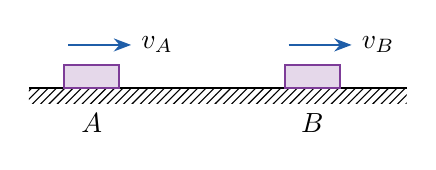
\begin{tikzpicture}[scale=1.0]
  \fill[pattern=north east lines] (-0.4,-0.2) rectangle (4.4,0);
  \draw[thick] (-0.4,0) -- (4.4,0);
  \foreach \x/\l/\v in {0.4/A/v_A, 3.2/B/v_B} {
    \filldraw[draw=morado, fill=morado!20, thick] (\x-0.35,0) rectangle (\x+0.35,0.3);
    \node[below] at (\x,-0.2) {$\l$};
    \draw[->, thick, azul] (\x-0.3,0.55) -- (\x+0.5,0.55) node[right, text=black]{$\v$};
  }
\end{tikzpicture}
\end{document}
